\section{Introduction}

\subsection{Basic matrix decomposition}

\subsubsection{LU factorization with (partial) pivoting}

If $A \in \mathbb{R}^{n\times n}$ is nonsingular (invertible), then
$$
    PA = LU
$$

\begin{itemize}
    \item $P$ is a permutation matrix
    \item $L$ is unit lower matrix
    \item $U$ is upper triangular
\end{itemize}


\textbf{\textit{Linear system solution}}:
$$
    A \mathbf{x} = \mathbf{b}
$$
\begin{enumerate}
    \item Factor $PA = LU$ (expensive, $O(n^{3})$)
    \item Solve $L\mathbf{y} = P \mathbf{b}$ (lower triangular system, $O(n^{2})$)
    \item Solve $U\mathbf{x} = \mathbf{y}$ (upper triangular system, $O(n^{2})$)
\end{enumerate}

\subsubsection{Cholesky decomposition}

If $A \in \mathbb{R}^{n \times n}$ is symmetric ($A^{T} = A$) and positive definite ($\mathbf{z}^{T}A \mathbf{z} > 0$ for all $\mathbf{z} \neq \mathbf{0}$), then
$$
    A = L^{T}L
$$
where $L$ is lower triangular (with positive entries on the diagonal).

\begin{tcolorbox}[title=Linear system solution]
    $$A \mathbf{x} = \mathbf{b}$$
    \begin{enumerate}
        \item Factor $A = L^{T} L$ (expensive, $O(N^{3})$)
        \item Solve $L^{T}\mathbf{y} = \mathbf{b}$ (lower triangular system, $O(n^{2})$)
        \item Solve $L \mathbf{x} = \mathbf{y}$ (upper triangular system, $O(n^{2})$)
    \end{enumerate}
\end{tcolorbox}

\subsubsection{QR decomposition}

If $A \in \mathbb{R}^{n \times n}$ is nonsingular (invertible), then
$$
    A = QR
$$
\begin{itemize}
    \item $Q$ is an orthogonal
    \item $R$ is upper triangular
\end{itemize}

\textbf{\textit{Linear system solution}}:

$$A\mathbf{x} = \mathbf{b}$$

\begin{enumerate}
    \item Factor $A = QR$ (expensive, $O(n^{3})$)
    \item Multiply $\mathbf{c} = Q^{T}\mathbf{b}$ ($O(n^{2})$)
    \item Solve $R\mathbf{x} = \mathbf{c}$ (lower triangular system, $O(n^{2})$)
\end{enumerate}

\subsection{Sparse matrices}

A sparse matrix is a matrix in which most elements are zero. Roughly speaking, given $A \in \mathbb{R}^{n\times n}$, the number of non-zero entries of $A$, called $\mathrm{nnz}(A)$, is $O(n)$.

Many matrices arising from real applications are sparse. If we need to store $A$, we can exploit the sparse structure using different \textbf{storage schemes}:

\begin{table}[h!]
    \centering
    \begin{tabular}{|l|c|r|}
        \hline
        Name             & Easy insertion & Fast $A \mathbf{x}$ \\
        \hline
        Coordinate (COO) & Yes            & No                  \\
        CSR              & No             & Yes                 \\
        \hline
    \end{tabular}
\end{table}

\subsubsection{Coordinate format (COO)}

The data structure consists of three arrays of length $\mathrm{nnz(A)}$:

\begin{itemize}
    \item \texttt{AA}:  all the values of the nonzero elements of $A$ \textit{in any order}
    \item \texttt{JR}: integer array containing their row indices
    \item \texttt{JC}: integer array containing their column indices
\end{itemize}

\textbf{\textit{Example}}

\begin{figure}[h]
    \centering
    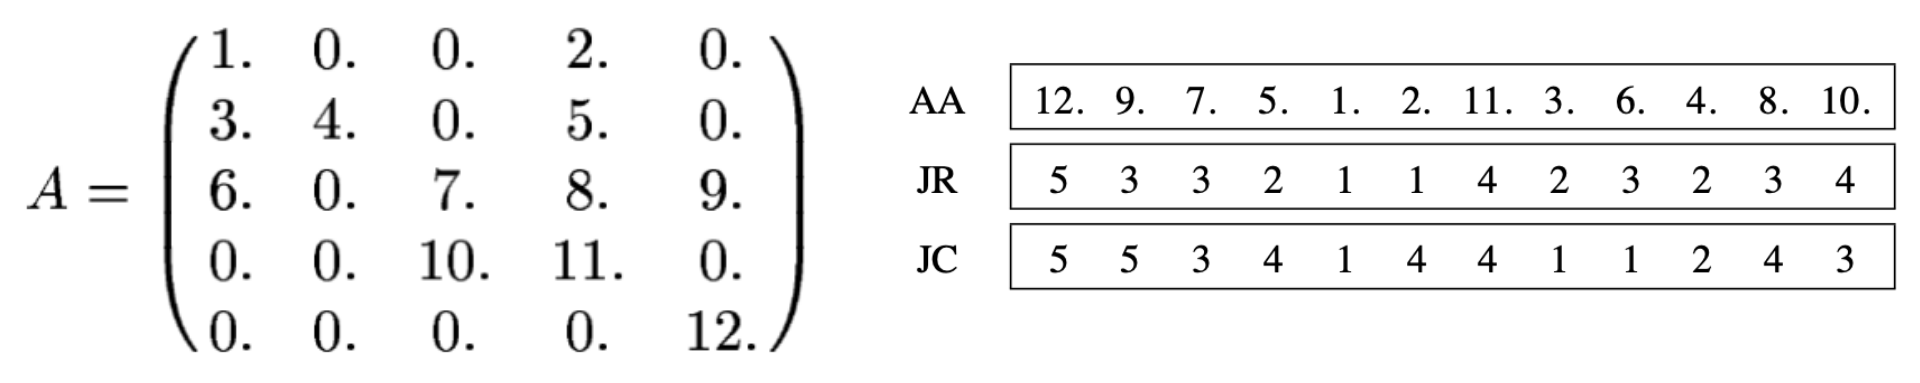
\includegraphics[width=0.75\textwidth]{images/example-coo.png}
\end{figure}

\subsubsection{Coordinate Compressed Sparse Row format (CSR)}

If the elements of $A$ are listed by row, the array \texttt{JC} might be replaced by an array that points to the beginning of each row.
\begin{itemize}
    \item \texttt{AA}: all the values of the nonzero elements of $A$, \textit{stored row by row} from $1, \dots, n$
    \item \texttt{JA}: contains the column indices
    \item \texttt{IA}: contains the pointers to the beginning of each row in the arrays \texttt{AA} and \texttt{JA}. Thus $IA(i)$ contains the position in the arrays \texttt{AA} and \texttt{JA} where the $i$-th row starts. The length of \texttt{IA} is $n + 1$.
\end{itemize}

\textbf{\textit{Example}}

\begin{figure}[h]
    \centering
    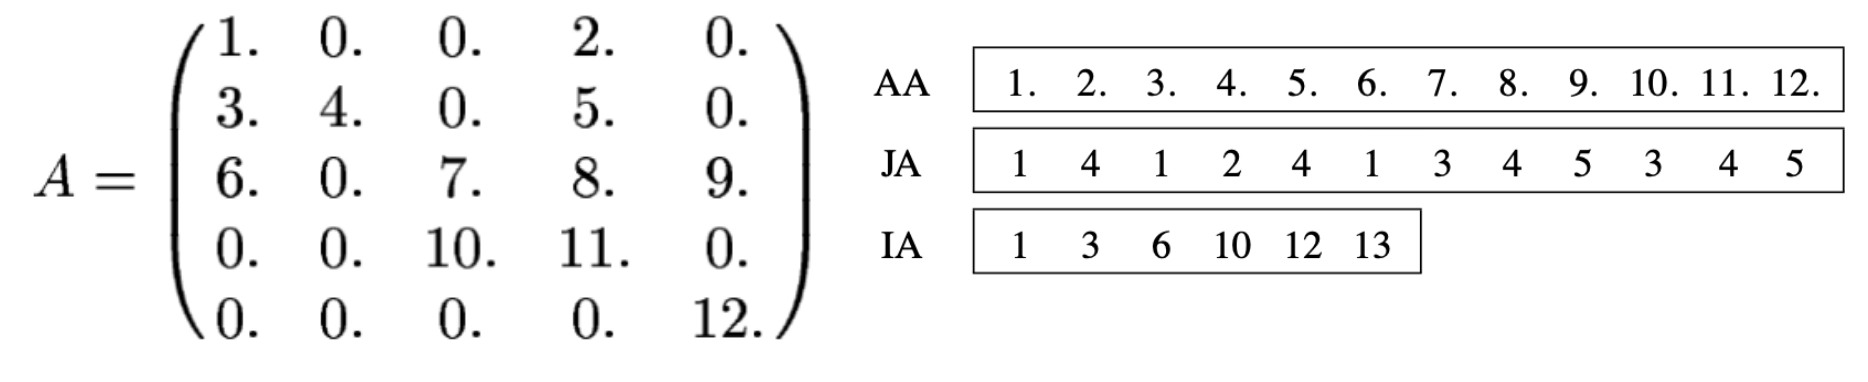
\includegraphics[width=0.75\textwidth]{images/example-csr.png}
\end{figure}
